%********** Chapter 7 **********
\chapter{Loop Closure and Global Optimization}
\section{Introduction}
As explained before, the alignment we are implementing is a pair-wise alignment which means that evey frame is aligned with the previous frame and so on, although this method gives good results, it will face a problem in case a loop happens in the scanning.

We explain this problem with a simple example:
Assume the user scanned a scene so five frames were aligned namely: A, B, C, D, E, If the user has returned to the starting point A then there will be overlapping between the first and last frames A and E respectively, the problem is that even if our alignment calculations are accurate, there are always small errors and false matches that accumlate all over the scanning process which will cause overlapping areas of A and E not to align perfectly as we would want, because we align E according to D only without considering the overlapping between the two frames A and E.

\pagebreak
We present here a visual explanation of the problem and examples of scanning processes that include loops.

\begin{figure}[H]
\centering
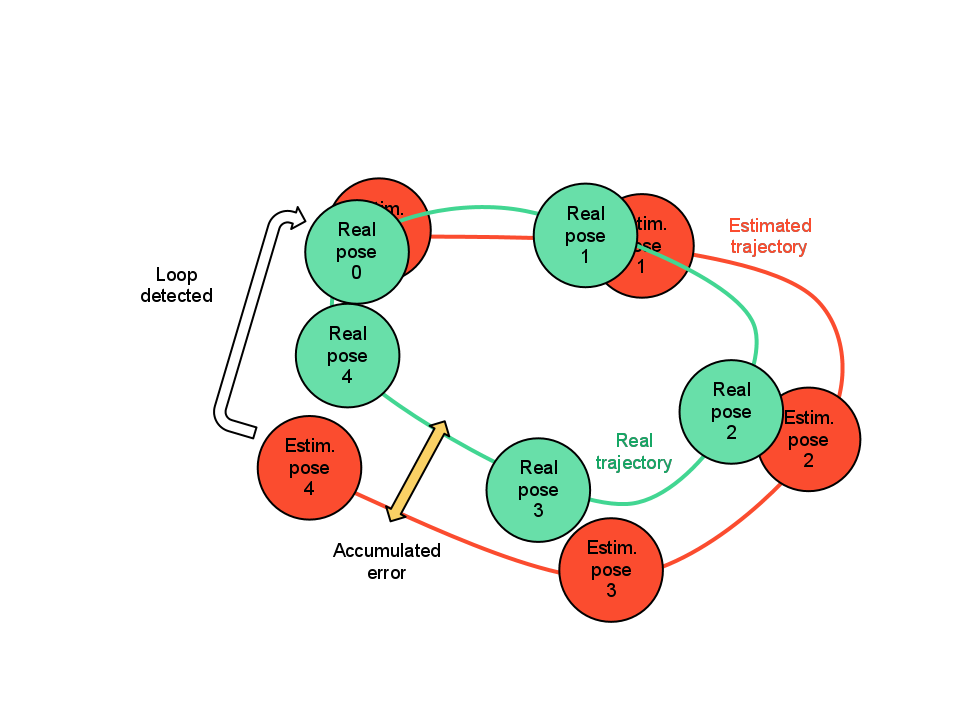
\includegraphics[scale=0.4,keepaspectratio=true]{Loop/loop_closure.png}
\caption{Because of accumlating alignment errors, the last estimated pose is far from where the real pose is}
\label{fig:loop_closure}
\end{figure}

\begin{figure}[H]
\centering
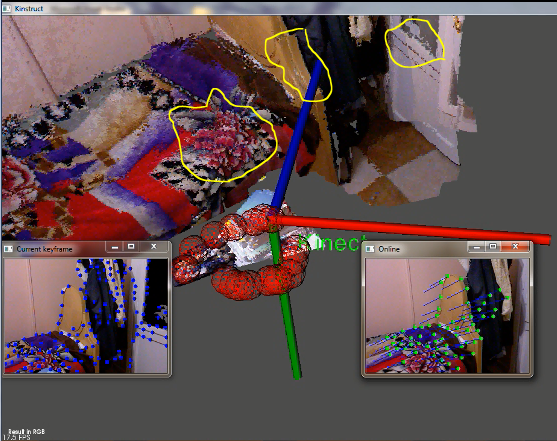
\includegraphics{Loop/last_frame_loop_highlighted.png}
\caption{Highlighted areas are duplicate objects that are not aligned as they should be because of accumlative numerical errors and false matches}
\label{fig:last_frame_loop_highlighted}
\end{figure}

Now that we have defined the problem, we introduce a solution that involves two steps; the first step is to detect that a loop has occured (user has returned to a previously visited scene), for the second step we try to realign the frames to remove the error in alignment between the first and last frames in the loop.

\pagebreak
\section{Loop Detection}

The brute force approach for loop detection is to just perform feature matching between the current frame and all previous frames and use a threshold to determine if a loop happened, this approach has two drawbacks:

\begin{itemize}
\item The overhead incurred for matching a frame with all previous frames is extremely high and is not acceptable for long scans especially that the system we are building is real-time system. 
\item This approach is not going to be conclusive in the case of similar scenes such as floors or repeated patterns because all the scanned frames will have high values for matching and we can't determine where the loop exactly was formed.
\end{itemize}

We enhanced the previous approach by performing feature matching only on frames that are spatially close to the current frame, this enhancement is achieved using a k-d tree holding all the previous pose estimations, then every new aligned frame is tested against only those frames that are within a certain distance from the current pose estimation.

\subsection{k-d Trees}
The data structure used to store the pose estimations must be optimized for spatial search, so we can find points that are in a certain range from another point, this is why we chose the k-d tree to store the pose estimations.

k-d is a space-partitioning data structure for organizing points in a k-dimensional space. k-d trees are a useful data structure for several applications, such as searches involving a multidimensional search key.


We explain here how a new point is inserted in a k-d tree, for simplicity we consider the case when k = 2 (each point has x and y coordinates), in this case we do insertion just like a binary tree but as we have two different values (x and y coordinates) at each node then we alternate between them in comparison; so we compare at the root according to x, then at depth one we compare according to y, then at depth two we compare according to x and so on ..

The following algorithm inserts a new node in a k-d tree where k = 2:\newline
\noindent procedure {\bf Insert(T, N, depth=0)} takes T the root of the tree, N the node to be inserted and depth holding the value of current depth.\newline
\noindent if T is NULL\newline
\indent then T = N \newline
else\linebreak
\indent if depth is even\newline
\indent \indent if N.x $>$ T.x \newline
\indent \indent \indent then Insert(T.right, N, depth + 1)\newline
\indent \indent else Insert(T.left, N, depth + 1)\newline
\indent else \newline
\indent \indent if N.y $>$ T.Y\newline
\indent \indent \indent Insert(T.right, N, depth + 1)\newline
\indent \indent else Insert(T.left, N, depth + 1)\newline


\begin{figure}[H]
\centering
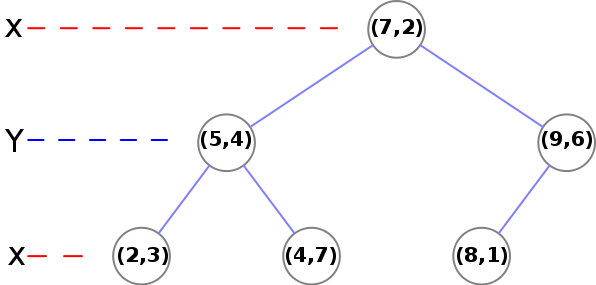
\includegraphics[scale=0.6,keepaspectratio=true]{Loop/kdtree_build_2.png}
\caption{k-d tree with d = 2, this tree was built by inserting (7,2), (9,6), (5,4), (2,3), (4,7) and (8,1)}
\label{fig:kdtree_build_2}
\end{figure}

\begin{figure}[H]
\centering
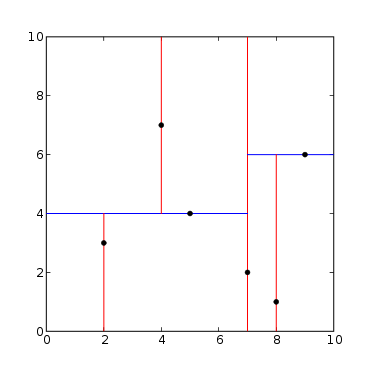
\includegraphics {Loop/kdtree_build_1.png}
\caption{The decompsition of the k-d tree in  fig ~\ref{fig:kdtree_build_2}}
\label{fig:kdtree_build_1}
\end{figure}

The previous procedure for building the k-d tree can be generalized fot k = 3 by alternating between x, y and z and each level of the tree.

After we have built the k-d tree containing all pose estimations, we need to find all the previous estimations that fall in a certain range from the current pose estimation.

\pagebreak
Range search operations in k-d tree depend on the fact that we partition the space into different parts, this is clear in the following figure:
\begin{figure}[H]
\centering
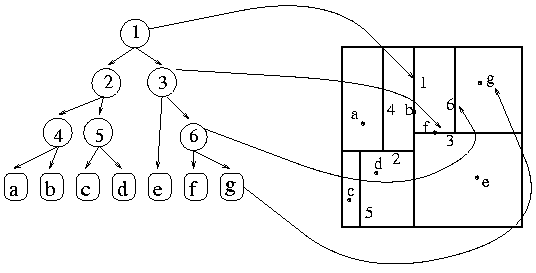
\includegraphics{Loop/k-d_tree_search1.png}
\caption{The root of the tree which is node 1 splits the space vertically into two parts; one containing all points on the left of point 1 and one containing all points on the right of point 1, the same is for node 3 which splites the space horizontally and node 6 that splits the space vertically }
\label{fig:k-d_tree_search1}
\end{figure}

The range search in k-d trees starts from the root and tests if any of its subtrees is fully contained inside the region then all nodes in the subtree are returned, if the subtree only intersects with the region then we call the search procedure on the subtree, but if the subtree is not contained and doesn't intersect with the region then we just ignore it.

\pagebreak
The following algorithm explains how search is performed:\newline
\noindent procedure {\bf SearchKdTree(v, R)} takes v the root of the tree, and R the range to search inside.

\noindent {\bf SearchKdTree( v, R )}\newline
\noindent if v lies in R\newline
\indent then Report the point stored at v \newline
else\linebreak
\indent if region( v.left ) is fully contained in R\newline
\indent \indent then ReportSubtree( v.left )\newline
\indent else\newline
\indent \indent if region( v.left ) intersects R\newline
\indent \indent \indent then SearchKdTree( v.left, R )\newline
\indent if region( v.right ) is fully contained in R\newline
\indent \indent then ReportSubtree( v.right )\newline
\indent else\newline
\indent \indent if region( v.right ) intersects R\newline
\indent \indent \indent then SearchKdTree( v.right, R )\newline

\begin{figure}[H]
\centering
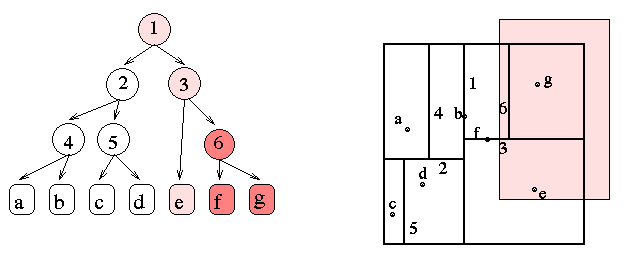
\includegraphics{Loop/k-d_tree_search2.png}
\caption{Here we search for any nodes that fall in the pink rectangluar, It is clear that the region rectangle intersects with the right side of point 1 and not with the left side of point 1, so we investigate only the right subtree starting at node 3, there we find that e the point below point 3 falls into the region and the subtree starting also intersects with the region so we investigate it and find that only the point g falls in the region}
\label{fig:k-d_tree_search2}
\end{figure}


\subsection{Feature matching}

After finding all previous pose estimations that fall in a certain range from the current previous estimation, we preform a visual test to make sure that the current pose and the previous one are both close to each other and are very similar visually.

We choose the closest pose estimation that is still far enough not to be just the previous one, and we use the feature matching explained before in chapter 4.

\begin{figure}[H]
\centering
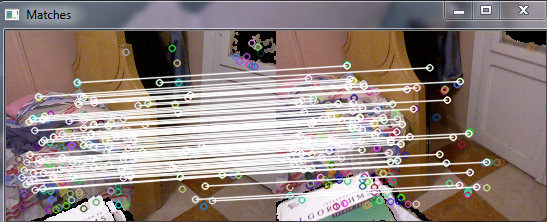
\includegraphics{Loop/loop_matches.png}
\caption{Feature matching between the first and last frame in the scanning }
\label{fig:first_frame_loop}
\end{figure}


\pagebreak
\subsection{Loop detection Results}

We present here three shots; the first shot represents the first frame of the scanning process and the first pose estimation indicated with the red sphere is at (0,0,0), the second shot shows the scene after building and the last frame is spatially close and visually similar to the first one so a loop is detected, the third shot shows us the loop in 3D space starting from (0,0,0) and going in anti clock-wise direction.

\begin{figure}[H]
\centering
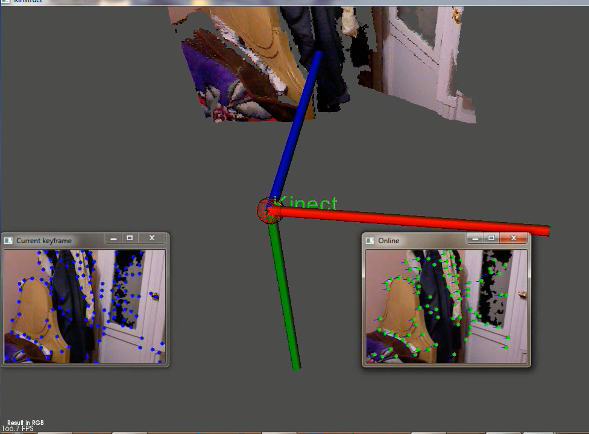
\includegraphics{Loop/first_frame_loop.png}
\caption{This is the first frame in a scanning process }
\label{fig:first_frame_loop}
\end{figure}

\begin{figure}[H]
\centering
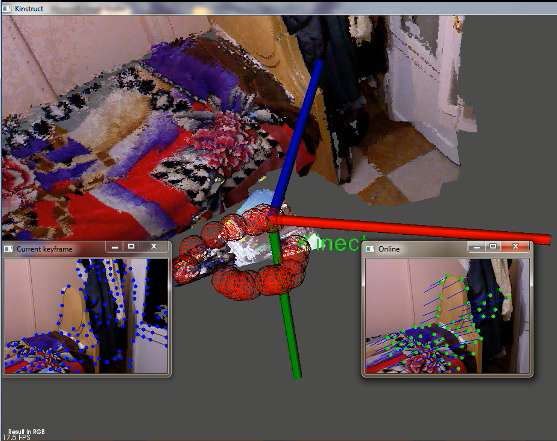
\includegraphics{Loop/last_frame_loop.png}
\caption{This is the last frame in scanning process, we notice that the last frame is similar to the first frame}
\label{fig:last_frame_loop}
\end{figure}

\begin{figure}[H]
\centering
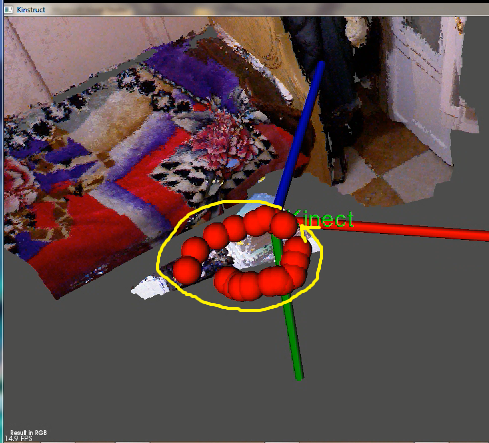
\includegraphics{Loop/loop.png}
\caption{The red spheres represent the pose estimations that form the loop}
\label{fig:loop}
\end{figure}

\pagebreak
\section{Global Optimization}

Now that we have been able to detect that a loop has occurred during the scan process, we need to find a way that will make the error in the loop has less effect on the constructed scene.

In SLAM graphs pose estimations are represented by nodes while edges represent constratints (transformations) between the estimations, the purpose of global optimization systesm is to minimize the global error in the graph by changing the constraints between the poses.

We have used the newly published method named Explicit Loop Closing heuristic, this method is different from other systems such as TORO that it is not an iterative method, the main idea of the algorithm is to dissociates the last scan of a sequence of acquired scans, reassociates it to the map, built so far by scan registration, and distributes the difference in the pose error over
the SLAM graph.

We used the implementation of which is provided as a part of the Point Cloud Library (PCL), the next section shows the results of loop detection followed by global optimization.

\pagebreak
\section{Implementaion and Results}

We have successfully used the techniques explained in previous sections to perform loop closure and global optimization, we have used a threshold of at most 15 cm between two frames to be considered spatially the same, then we require at least 10 SURF feature matches between the two frames to be visually the same.

We present here two shots of the same constructed scene before and after the applying ELCH to remove noise and duplication resulting from loop closure and accumlating error, the fixing operation took about 16 seconds for 18 aligned frames with QVGA quality.

\begin{figure}[H]
\centering
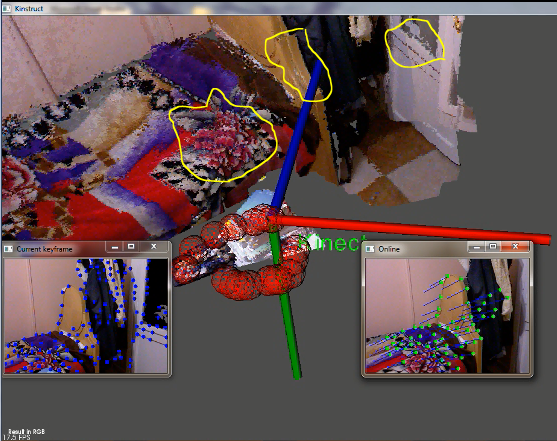
\includegraphics{Loop/last_frame_loop_highlighted.png}
\caption{Highlighted areas are duplicate objects that are not aligned as they should be because of accumlative numerical errors and false matches}
\label{fig:before_fixing}
\end{figure}

\begin{figure}[H]
\centering
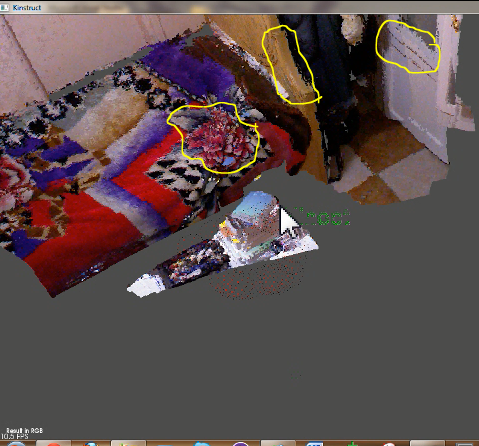
\includegraphics{Loop/after_fixing.png}
\caption{After applying ELCH, we notice how noise and duplication from the marked area compared with the constructed scene before applying ELCH in fig ~\ref{fig:before_fixing} }
\label{fig:after_fixing}
\end{figure}
